\section{Algoritme til detektering af gang, løb og cykling}
\textit{Dette afsnit omhandler design, implementering og test af algoritmerne til detektering af gang, løb og cykling. Først bliver design af algoritmerne behandlet, hvilket er ensbetydende med at implementering og kodning kan foregå. Når algoritmerne er designet og implementeret bliver de efterfølgende testet for at af- eller bekræfte deres virkning.}

\subsection{Design}
For at kunne adskille gang, løb og cykling benyttes et accelerometer og et gyroskop som er beskrevet i \secref{LSM9DS1}\fxnote{opg: tjek op på denne reference}. Herunder vil gyroskopet blive benyttet til at detektere cykling, mens løb og gang detekteres ved brug af accelerometeret. For at kunne detektere og adskille disse aktiviteter, behandles inputtet fra sensorerne gennem forskellig signalbehandling, hvorefter algoritmer afgør om de pågældende signaler repræsenterer gang, løb, cykling eller ingen aktivitet. 


\subsubsection{Gang og løb}
Data fra accelerometerets y-akse skal signalbehandles, førend en algoritme kan detektere og adskille gang fra løb. Første trin i denne signalbehandling er, at fjerne støj ved brug af et elliptisk filter. Dette skal være et elliptisk 4. ordens båndpasfilter med et pasbånd fra 20 til 50 Hz, og med en dæmpningsgrad på 60 dB\fxnote{og 0.5 dB peak-to-peak ripples}. Båndpasfilterets knækfrekvenser er tildels bestemt gennem pilotforsøget. Knækfrekvensen omkring 20 Hz er enebestemmende for at bibeholde signalets hælnedslag, hvoraf frekvensen befandt sig omkring 20 Hz. Knækfrekvensen omkring 50 Hz er bestemt ligeledes bestemt på baggrund af pilotforsøget, hvoraf signalets frekvensindhold stopper herefter. Andet trin i signalbehandlingen, består af, at det filtrede signal divideres to. Dette er tilfældet da signalets amplituder bliver formindsket, og de mindste amplituder nærmer sig nul i større grad end hælnedslaget. Tredje trin i signalbehandlingen består i at det filtrerende og dividerede signal bliver kvadreret. Resultatet heraf medfører at amplituder som er lave ikke forstærkes i stor grad, og større amplituder forstærkes i stor grad. Dermed minimeres events som ikke relateres til hælnedslaget kraftigt, og selve hælnedslaget forstærkes.\fxnote{ved gang er det swing og heel strike, ved løb er det primært kun heel strike, men også lidt toe offset.} Fjerde og sidste trin i signalbehandlingen, bliver signalet filtreret med et moving average filter som udglatter signalet, hvilket resulterer i at små udslag ikke opfattes, og signalets hælnedslag vil fremstå som et enkelt event. \\

Førend ovenstående signalbehandling kan overføres til at fastsætte en tærskelværdi skal dataet fra pilotforsøgets data omregnes til LSM9DS1' arbejdsområde: 
\begin{equation}
\frac{32 g \cdot 2^{16}}{32 g \cdot 2^{12}} = 16
\end{equation}
Data fra Shimmer3 samples med en 12 bit ADC, og LSM9DS1 indebærer en 16 bit ADC. Resultatet heraf er at data fra pilotforsøgets skal ganges med 16 for at repræsenterer LSM9DS1' arbejdsområde.

Resultatet af ovenstående signalbehandling medfører at der findes et udtryk for gang og løbs amplitude forhold. Ud fra denne behandling af pilotforsøgets data vurderes det, at amplituden for hælnedslag ved løb overstiger 1100 og ved gang overstiger 50, hvorfor events med amplituder under 50 ikke vurderes som værende aktivitet.

\begin{figure}[H]
	\centering
	\includegraphics[scale=0.5]{figures/cDesign/algoritme_gl.png}
	\caption{Flowchart over algoritmen til detektering af gang og løb}
	\label{fig:algoritme}
\end{figure}

Ovenstående figur repræsenterer algoritmen for detektering og adskilles af gang og løb. Førend algoritmen tilhørende gang og løb starter, undersøges hvorvidt cykling registreres. Hvis dette ikke er tilfældet og løb detekteres, skal en timer stoppe når løb ikke længere detekteres. Når timeren stopper gemmes varigheden for timeren i et array tilhørende udført løb og max peak registreres og gemmes ligeledes. Herefter startes timeren igen. Hvis løb ikke detekteres, undersøges der hvorvidt gang registreres. Hvis gang registreres skal en timer ligeledes først stoppe når gang ikke længere detekteres. Når timeren stopper gemmes varigheden for timeren i et array tilhørende udført gang og max peak registeres og gemmes ligeledes. Herefter startes timeren igen. Hvis algoritmen for detektering af løb og gang ikke registrer aktiviteterne, så bliver der ikke udført nogen bevægelse, og algoritmen starter forfra.

\subsection{Cykling}
Data fra gyroskopets z-akse skal signalbehandles, førend en algoritme kan detektere og adskille aktiviteterne. Første trin i denne signalbehandling er at udføre en Fast Fourier Transform (FFT) over fire sekunders sampling. Dette medfører at signalets magnitude og dets tilhørende frekvenser kommer til udtryk, hvorefter andet trin indledes. Dette trin finder den maksimale magnitude med tilhørende frekvens. Tredje trin består af to summeringer, første summering summerer FFT'en fra den frekvens hvor den største magnitude befandt sig $\pm$1 Hz. Anden summering summerer FFT'en fra 1 til 20 Hz. Resultaterne af disse, benyttes til fjerde og sidste trin, som omregner hvor stor en procentdel den første summering udgør af den anden summering. \\
Resultatet af ovenstående signalbehandling medfører at der opstilles et udtryk for signalets spredning af energi. Det gør sig gældende at cykling har en spredning af energi fordelt nært frekvensen med den største amplitude. Data fra gyroskopets z-akse vedrørende cykling blev for alle forsøgspersoner, behandlet med ovenstående metode. Dette resulterede i at 84,5\% til 91,9\% af energien lå $\pm$1 Hz omkring den fundne frekvens. Følgende blev ligeledes behandlet for gang og løb, for at sikre disse ikke havde samme spredning i frekvensområdet, hvormed en mulig tærskelværdi til detektering af cykling, kan fastsættes.  Dette resulterede i at ved gang befandt energien omkring den fundne frekvens sig mellem 35,9\% til 48,5\% og ved løb befandt energien omkring den fundne frekvens sig mellem 42,8\% til 60,5\%. \\
Resultatet af at energien omkring den fundne frekvens med den største amplitude er $\approx$30\% større ved cykling end ved gang og løb, fastsættes tærskelværdien til 70\%. For at detektere cykling skal outputtet fra databehandlingen være større end 70\%.

\begin{figure}[H]
	\centering
	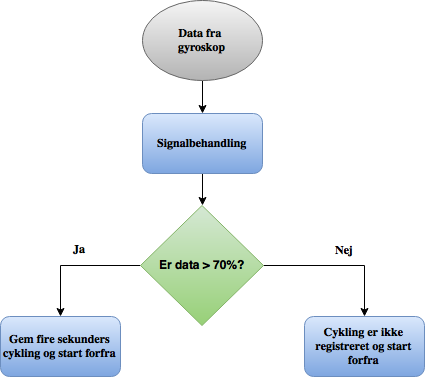
\includegraphics[scale=0.6]{figures/cDesign/algoritme_cykling.png}
	\caption{På figuren ses et flowchart som gennemgår algoritmen vedrørende detektering af cykling. \textbf{DETTE SKAL LAVES OM EFTER VI HAR LAVET ALGORITMEN}}
	\label{fig:algoritme_cykling}
\end{figure}

Ovenstående figur repræsenterer algoritmen for detektering af cykling. Hvis cykling detekteres skal en counter starte og først stoppe når cykling ikke længere detekteres. Når counteren stopper gemmes varigheden af counteren i et array tilhørende udført cykling. Hvis cykling ikke detekteres skal gyroskopet gå i LPM i 10 sekunder før algoritmen køres igen. 


\subsection{Implementering}
\subsubsection{Gang og løb}
Implementeringen af algoritmen for detektering af gang og løb består grundlæggende af to delelementer. Først signalbehandling, hvorefter selve algoritmen implementeres- Signal behandlingen er blevet implementeret som enestående funktioner, hvoraf signalet bliver behandlet med fire funktion førend data bliver behandlet med algoritmen. \\
Igennem design blev det bestemt at signalet først skal filtreres med et elliptisk båndpasfilter. Dette blev implementeret på MCU'en som et IIR filter, med filterkoefficienter udregnet gennem MATLAB. Derefter blev signalet divideret, kvadreret og moving average filtreret. 

\begin{figure}[H]
	\centering
	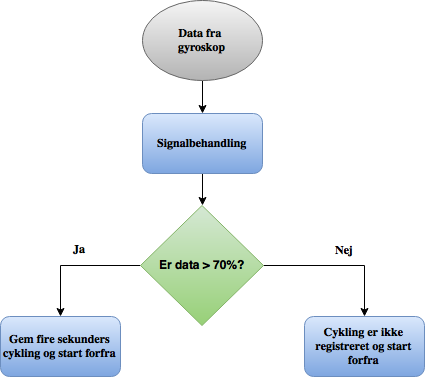
\includegraphics[scale=0.6]{figures/cDesign/algoritme_cykling.png}
	\caption{På figuren ses et flowchart som gennemgår algoritmen vedrørende detektering af cykling. \textbf{DETTE SKAL LAVES OM EFTER VI HAR LAVET ALGORITMEN}}
	\label{fig:algoritme_cykling}
\end{figure}

bla 





Interrupt service rutiner

Det elliptiske filter er lavet som et IIR filter, ud fra filterkoefficienter fra matlab.




\subsection{Test}

Shimmer data ganges med 16


Test filter:\\
- Lav en rx-tx forbindelse mellem PS og PSoC\\
- send et hvid-støj signal ind (indeholder alle frekvenser)\\
- Det vi får tilbage bør kun indeholde de frekvenser vi gerne vil have/have dæmpet udenfor pasbåndet. \\

eller send en sinus ind med en given frekvens (5 Hz), tjekker dæmpning af den givne frekvens\\

signal m hvid støj : help rand --> "rand" genererer hvid støj\\











%%%%%%%%%%%%

Rettelser:
løb = >2.5
gang = 2.5 > 0.5
